\section{Le problème de flot à coût minimum (PFCM)}

Un très grand nombre de programmes linéaires possèdent une composante ``réseau'' très importante.
Nous allons étudier dans cette section le problème consistant à approvisionner, au moindre coût, des entrepôts à partir des unités de production (usines) d'une compagnie.
Les données du problème sont:
\begin{itemize}
\item
le réseau de transport;
\item
la localisation et la capacité de production des usines (sources);
\item
la localisation et la demande des entrepôts (destinations);
\item
les coûts de transport $c_{ij}$ sur les arcs du réseau.
\end{itemize}
Il reste à déterminer les productions des usines ainsi que les chemins utilisés pour approvisionner les entrepôts.
Désignons par $b_i$ la demande associée au sommet $i$.
Par convention, un sommet d'offre (usine) possède une demande négative et un sommet de passage (ni usine ni entrepôt) possède une demande nulle.
Pour simplifier, nous supposerons que l'offre est égale à la demande, c'est-à-dire:
\[
\sum_i b_i = 0.
\]
Il semble naturel de formuler ce problème en terme de flots sur les chemins reliant les sources et les destinations du résau.
Or, le nombre de chemins étant astronomique, il est plus simple d'utiliser les flots
sur les arcs comme variables, quitte à récupérer les flots de chemins par la suite.
Soit $x_{ij}$ le flot sur l'arc $(i, j)$.
De façon naturelle, les flots doivent être non négatifs.
Ils doivent également satisfaire aux conditions de conservation qui stipulent que le flot ne peut être créé qu'aux sources et absorbé aux destinations.
En tout autre sommet du réseau, le flot entrant doit correspondre au flot sortant.

Le PFCM prend ainsi la forme du programme linéaire
\[
\min_{x \in \XX} cx,
\]
où
\[
\XX = \left\lbrace
x \geq 0 \mbox{ t.q. } \sum_j x_{ji} - \sum_j x_{ij} = b_i,\ \forall i \in \NN \right\rbrace
= \lbrace x \geq 0 \mbox{ t.q. } Ax = b \rbrace.
\]

Considérons le réseau représenté sur la Figure~\ref{fig:pfcm}.
La matrice A représente la matrice d'incidence sommets-arcs du graphe.
Chaque colonne décrit un arc alors que la ligne $i$ contient l'information pertinente au sommet $i$.
\begin{align*}
A & =
\begin{pmatrix}
-1 & -1 & -1 \\
+1 & & & -1 & -1 \\
& +1 & & & & -1 & +1 \\
& & & +1 & & +1 & & +1 \\
& & +1 & & +1 & & -1 & -1
\end{pmatrix} \\
b & =
\begin{pmatrix}
-5 \\
-3 \\
+2 \\
+6 \\
0
\end{pmatrix}
\qquad
c = ( 1, 10, 3, 7, 9, -3, 4, 2 ).
\end{align*}

\begin{figure}[htbp]
\begin{center}
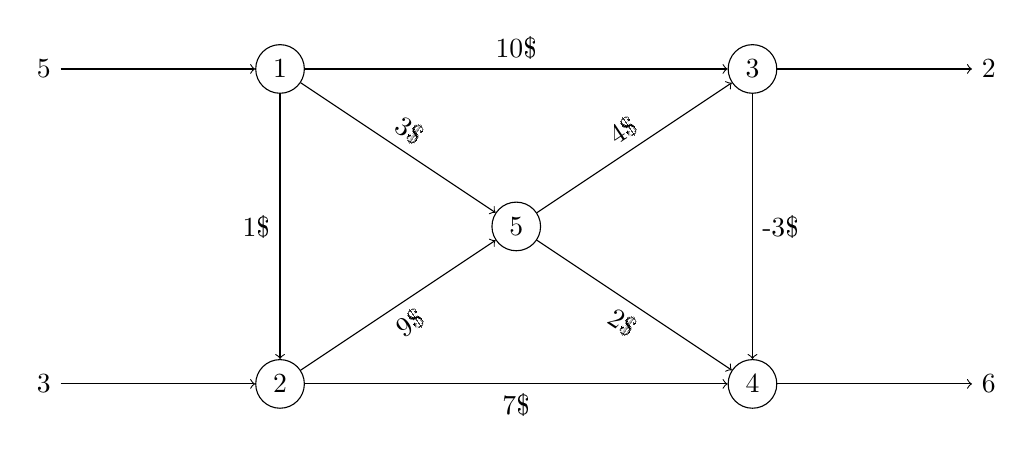
\begin{tikzpicture}
\node
(1i) at (1,4) {5};
\node
(2i) at (1,0) {3};
\node
(3o) at (13,4) {2};
\node
(4o) at (13,0) {6};
\node[circle,draw]
(1) at (4,4) {1};
\node[circle,draw]
(2) at (4,0) {2};
\node[circle,draw]
(3) at (10,4) {3};
\node[circle,draw]
(4) at (10,0) {4};
\node[circle,draw]
(5) at (7,2) {5};
\draw[->](1i) -- (1);
\draw[->](2i) -- (2);
\draw[->](3) -- (3o);
\draw[->](4) -- (4o);
\draw[->](1) -- (2) node[left,midway] {1\$};
\draw[->](1) -- (3) node[above,midway] {10\$};
\draw[->](1) -- (5) node[sloped,above,midway] {3\$};
\draw[->](2) -- (4) node[below,midway] {7\$};
\draw[->](2) -- (5) node[sloped,below,midway] {9\$};
\draw[->](3) -- (4) node[right,midway] {-3\$};
\draw[->](5) -- (3) node[sloped,above,midway] {4\$};
\draw[->](5) -- (4) node[sloped,below,midway] {2\$};
\end{tikzpicture}
\caption{Exemple de PFCM}
\label{fig:pfcm}
\end{center}
\end{figure}

Ce programme étant linéaire, il est naturel de lui appliquer l'algorithme du simplexe. Celui-ci prend une forme très particulière sur les réseaux.
Sans entrer dans les détails techniques, mentionnons qu'un point extrémal (solution de base) est obtenu en affectant le flot uniquement sur un arbre du réseau touchant à
tous les sommets.
A chaque arbre correspond une et une seule affectation du flot qui satisfait aux offres
et aux demandes du problème.

On introduit, à chaque sommet $i$, un nombre $y_i$ représentant la longueur de l'unique chemin allant de la racine au sommet $i$ dans l'arbre.
Si un arc est utilisé à rebours, son coût change de signe.
La distance entre deux sommets $i$ et $j$ du réseau, en passant par l'arbre, est alors $y_j - y_i$.